\documentclass[border=10pt]{standalone}
\usepackage{amsmath}
\usepackage{tikz}
\usetikzlibrary{positioning, arrows.meta, calc, fit, backgrounds, shapes.geometric}
\begin{document}
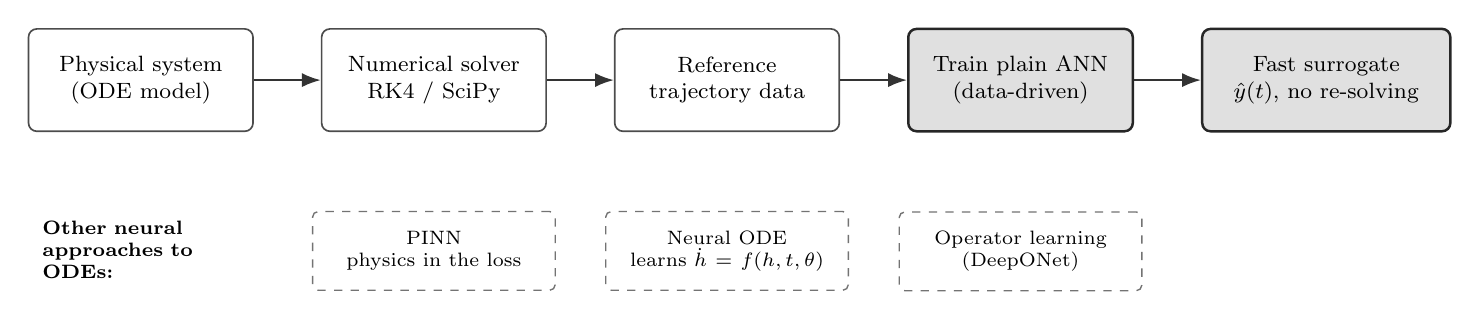
\begin{tikzpicture}[
    font=\footnotesize, node distance=0.8cm and 0.85cm,
    stage/.style={rounded corners=3pt, draw=black!70, fill=white, line width=0.6pt,
                  align=center, inner sep=5pt, text width=2.5cm, minimum height=1.3cm},
    nn/.style={rounded corners=3pt, draw=black!85, fill=black!12, line width=0.9pt,
               align=center, inner sep=5pt, text width=2.5cm, minimum height=1.3cm},
    outbox/.style={rounded corners=3pt, draw=black!85, fill=black!12, line width=0.9pt,
                align=center, inner sep=5pt, text width=2.8cm, minimum height=1.3cm},
    chip/.style={rounded corners=2pt, draw=black!55, fill=white, line width=0.5pt, dashed,
                 align=center, inner sep=4pt, text width=2.8cm, font=\scriptsize, minimum height=1.0cm},
    flow/.style={-{Latex[length=2.4mm]}, line width=0.8pt, draw=black!80}
]
\node[stage] (sys) {Physical system\\(ODE model)};
\node[stage, right=of sys] (solv) {Numerical solver\\RK4 / SciPy};
\node[stage, right=of solv] (data) {Reference\\trajectory data};
\node[nn, right=of data] (train) {Train plain ANN\\(data-driven)};
\node[outbox, right=of train] (surr) {Fast surrogate\\$\hat{y}(t)$, no re-solving};
\foreach \a/\b in {sys/solv, solv/data, data/train, train/surr}{\draw[flow] (\a)--(\b);}
\node[align=left, font=\scriptsize, text width=2.5cm, below=1.0cm of sys] (lbl)
      {\textbf{Other neural}\\\textbf{approaches to ODEs:}};
\node[chip, below=1.0cm of solv] (pinn) {PINN\\physics in the loss};
\node[chip, below=1.0cm of data] (nodeb) {Neural ODE\\learns $\dot{h}=f(h,t,\theta)$};
\node[chip, below=1.0cm of train] (op) {Operator learning\\(DeepONet)};
\end{tikzpicture}
\end{document}
